\documentclass[12pt]{article}
\usepackage{amsmath}
\usepackage{amsfonts}
\usepackage{amssymb}
\usepackage{tikz}
\usetikzlibrary{arrows.meta}

\begin{document}

\begin{center}
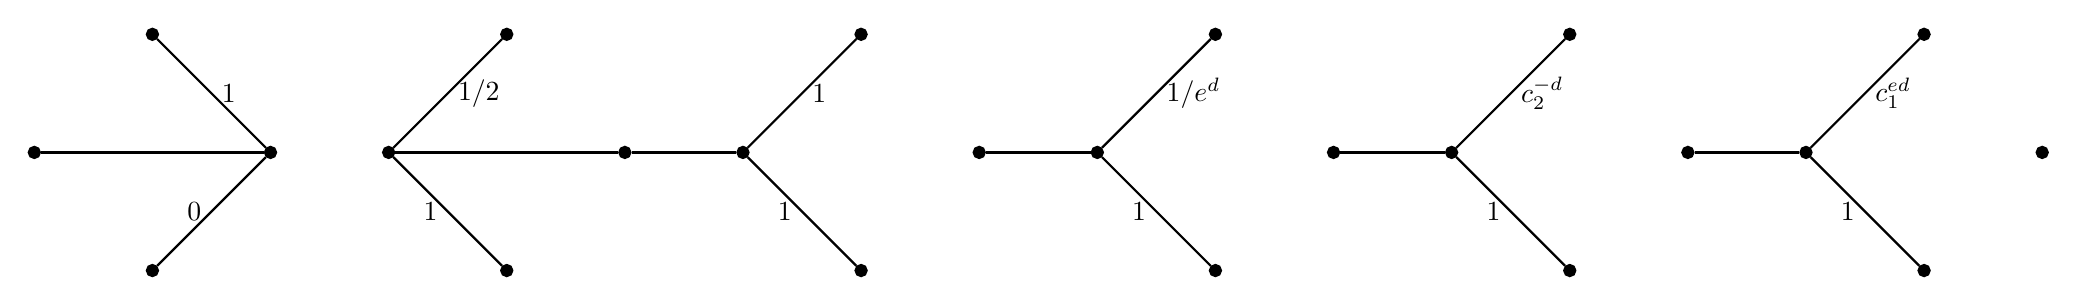
\begin{tikzpicture}[thick, scale=0.5]
  \tikzstyle{vertex}=[draw,circle,fill=black,minimum size=4pt,inner sep=0pt]

  \node[vertex] at (-3,0) (v11) {};
  \node[vertex] at (-6,-3) (v12) {};
  \node[vertex] at (-6,3) (v13) {};
  \node[vertex] at (-9,0) (v21) {};

  \draw (v11)--node[left]{$0$}(v12);
  \draw (v11)--node[right]{$1$}(v13);

  \draw (v21)--(v11);

  \node[vertex] at (0,0) (v31) {};
  \node[vertex] at (3,-3) (v32) {};
  \node[vertex] at (3,3) (v33) {};
  \node[vertex] at (6,0) (v41) {};

  \draw (v31)--node[left]{$1$}(v32);
  \draw (v31)--node[right]{$1/2$}(v33);
  \draw (v31)--(v41);

  \node[vertex] at (9,0) (v51) {};
  \node[vertex] at (12,-3) (v52) {};
  \node[vertex] at (12,3) (v53) {};
  \node[vertex] at (15,0) (v61) {};

  \draw (v51)--node[left]{$1$}(v52);
  \draw (v51)--node[right]{$1$}(v53);

  \draw (v41)--(v51);

  \node[vertex] at (18,0) (v71) {};
  \node[vertex] at (21,-3) (v72) {};
  \node[vertex] at (21,3) (v73) {};
  \node[vertex] at (24,0) (v81) {};

  \draw (v71)--node[left]{$1$}(v72);
  \draw (v71)--node[right]{$1/e^d$}(v73);

  \draw (v61)--(v71);

  \node[vertex] at (27,0) (v91) {};
  \node[vertex] at (30,-3) (v92) {};
  \node[vertex] at (30,3) (v93) {};
  \node[vertex] at (33,0) (v101) {};

  \draw (v91)--node[left]{$1$}(v92);
  \draw (v91)--node[right]{$c_2^{-d}$}(v93);

  \draw (v81)--(v91);

  \node[vertex] at (36,0) (v111) {};
  \node[vertex] at (39,-3) (v112) {};
  \node[vertex] at (39,3) (v113) {};
  \node[vertex] at (42,0) (v121) {};

  \draw (v111)--node[left]{$1$}(v112);
  \draw (v111)--node[right]{$c_1^{e d}$}(v113);

  \draw (v101)--(v111);
\end{tikzpicture}
\end{center}

Increasing the input capacities may result in reduced effective throughputs on some inputs, as if they are in competition. Similarly, increasing the output capacities may also result in reduced effective throughputs on some outputs.